\documentclass[paper=a4, fontsize=11pt]{scrartcl} % A4 paper and 11pt font size

\usepackage[T1]{fontenc} % Use 8-bit encoding that has 256 glyphs
\usepackage{fourier} % Use the Adobe Utopia font for the document - comment this line to return to the LaTeX default
\usepackage[english]{babel} % English language/hyphenation
\usepackage{amsmath,amsfonts,amsthm} % Math packages
\usepackage{graphicx}
\usepackage{booktabs}
\usepackage{float}

\usepackage{lipsum} % Used for inserting dummy 'Lorem ipsum' text into the template

\usepackage{sectsty} % Allows customizing section commands
\allsectionsfont{\centering \normalfont\scshape} % Make all sections centered, the default font and small caps

\usepackage{color} % or xcolor
\usepackage{soul}

\usepackage{fancyhdr} % Custom headers and footers
\pagestyle{fancyplain} % Makes all pages in the document conform to the custom headers and footers
\fancyhead{} % No page header - if you want one, create it in the same way as the footers below
\fancyfoot[L]{} % Empty left footer
\fancyfoot[C]{} % Empty center footer
\fancyfoot[R]{\thepage} % Page numbering for right footer
\renewcommand{\headrulewidth}{0pt} % Remove header underlines
\renewcommand{\footrulewidth}{0pt} % Remove footer underlines
\setlength{\headheight}{13.6pt} % Customize the height of the header

\numberwithin{equation}{section} % Number equations within sections (i.e. 1.1, 1.2, 2.1, 2.2 instead of 1, 2, 3, 4)
\numberwithin{figure}{section} % Number figures within sections (i.e. 1.1, 1.2, 2.1, 2.2 instead of 1, 2, 3, 4)
\numberwithin{table}{section} % Number tables within sections (i.e. 1.1, 1.2, 2.1, 2.2 instead of 1, 2, 3, 4)

\setlength\parindent{0pt} % Removes all indentation from paragraphs - comment this line for an assignment with lots of text

\newtheorem{definition}{Definition}
\newtheorem{theorem}{Theorem}

\graphicspath{{./}{Girko/}{geff/}{oja_chaos/}{network_analysis/}{signal_comparison/}}

%----------------------------------------------------------------------------------------
%	TITLE SECTION
%----------------------------------------------------------------------------------------

\newcommand{\horrule}[1]{\rule{\linewidth}{#1}} % Create horizontal rule command with 1 argument of height

\title{
\normalfont \normalsize
\textsc{Princeton University, Applied Dynamical Systems} \\ [25pt] % Your university, school and/or department name(s)
\horrule{0.5pt} \\[0.4cm] % Thin top horizontal rule
\huge Oja-Type Plasticity and Neural Signal Reconstruction in Recurrent Networks  \\ % The assignment title
\horrule{2pt} \\[0.5cm] % Thick bottom horizontal rule
}

\author{David Hovey \& Aditya Biswas} % Your name

\date{\normalsize\today} % Today's date or a custom date

\begin{document}

\maketitle % Print the title

%----------------------------------------------------------------------------------------
%	INTRODUCTION
%----------------------------------------------------------------------------------------

\section{Introduction}
% TODO: Write at end once all sections are finalized.

%----------------------------------------------------------------------------------------
%	MOTIVATION
%----------------------------------------------------------------------------------------

\section{Motivation}
% TODO: Adi — mention reservoir computing and the biological motivation for studying
% structured rhythmic input in the context of seizure-like synchrony.

Neural circuits must represent time-varying signals — sensory inputs, motor rhythms,
and internally generated oscillations — using populations of neurons whose collective
activity can be understood as a high-dimensional dynamical trajectory.  A key empirical
observation is that healthy neural computation tends to exploit a large fraction of the
available state space: different stimuli or behavioral contexts engage different
combinations of neurons, and the population activity lives in a relatively
high-dimensional subspace.  Seizure-like states break this pattern.  During pathological
hypersynchrony, many neurons fire together, the activity collapses toward a
low-dimensional attractor, and the representational capacity of the circuit is severely
reduced.

This raises a natural question for computational neuroscience: can a simple, local
synaptic learning rule — one that modifies weights based only on the pre- and
postsynaptic activity of the neurons it connects — drive a recurrent network toward or
away from this kind of low-dimensional synchrony?  We study Oja-type plasticity, a
biologically plausible Hebbian rule with activity-dependent normalization, operating
on a randomly initialized recurrent network driven by periodic input.

%----------------------------------------------------------------------------------------
%	BACKGROUND
%----------------------------------------------------------------------------------------

\section{Background}

\subsection{Fixed-Weight Recurrent Networks}

A standard model of a recurrent neural network with fixed connectivity is the
continuous-time firing-rate equation

\begin{equation}
    \tau \dot{x}_i = -x_i + f\!\left(\sum_j W_{ij} x_j + b_i\right),
    \label{eq:rnn}
\end{equation}

where $x_i(t) \in \mathbb{R}$ is the activity of neuron $i$, $\tau > 0$ is the
membrane time constant, $W_{ij}$ is the synaptic weight from neuron $j$ to neuron $i$,
$b_i$ is a fixed external input or bias, and $f$ is a bounded nonlinear activation
function (here $f = \tanh$).  In vector form, \eqref{eq:rnn} is

\begin{equation}
    \tau \dot{\mathbf{x}} = -\mathbf{x} + f(W\mathbf{x} + \mathbf{b}).
\end{equation}

For fixed $W$, the long-term behavior of the system — fixed points, limit cycles,
and chaos — is determined by the interplay between the weight spectrum and the
nonlinear saturation of $f$.  This fixed-weight setting is the classical starting
point for reservoir computing \cite{sompolinsky1988chaos}, in which the recurrent
network acts as a high-dimensional nonlinear filter and a linear readout is
trained to extract the desired signal from the activity.

\subsection{Grossberg \(S\)-\(\Sigma\) Equivalence}

An alternative but equivalent formulation of \eqref{eq:rnn}, common in
Grossberg-type models, separates the nonlinearity from the summation:

\begin{equation}
    \tau \dot{x}_i = -x_i + \sum_j W_{ij} S(x_j) + b_i,
\end{equation}

where $S(x_j)$ is interpreted as the nonlinear signal emitted by the presynaptic
neuron $j$, which is then weighted by $W_{ij}$ and integrated by the postsynaptic
neuron $i$.  In the standard formulation \eqref{eq:rnn}, the nonlinearity is applied
\emph{after} summation; in the $S$-$\Sigma$ formulation it is applied \emph{before}.
When $f = S$, the two are formally identical, which can be seen by identifying
$f(\sum_j W_{ij} x_j + b_i)$ with $\sum_j W_{ij} S(x_j) + b_i$ up to the
placement of the nonlinearity relative to the weighted sum.  Throughout this paper
we use the standard post-summation form \eqref{eq:rnn}, but the Grossberg
perspective will be useful when interpreting the presynaptic activity $S(x_j) =
\tanh(x_j)$ as the signal that drives synaptic modification.

\subsection{Learning in Recurrent Neural Networks}

Introducing synaptic plasticity makes the weights $W_{ij}(t)$ dynamic, so the
full system evolves in the enlarged state space $(\mathbf{x}(t), W(t))$.  A
standard local model of synaptic modification is Hebbian learning,

\begin{equation}
    \dot{W}_{ij} = \eta\, x_i x_j,
\end{equation}

which increases $W_{ij}$ when the presynaptic activity $x_j$ and the postsynaptic
activity $x_i$ are positively correlated.  Hebbian learning alone leads to
unbounded growth of the weights whenever the network is driven by a consistent
signal.

Oja's rule \cite{sompolinsky1988chaos} stabilizes Hebbian learning by adding an
activity-dependent normalization term:

\begin{equation}
    \dot{W}_{ij} = \eta\, x_i x_j - \eta\, x_i^2 W_{ij}.
\end{equation}

We study the extended version with an additional weight-decay term:

\begin{equation}
    \dot{W}_{ij} = \eta\, x_i(x_j - x_i W_{ij}) - \lambda W_{ij},
    \label{eq:oja}
\end{equation}

where $\eta > 0$ is the learning rate and $\lambda > 0$ is the decay coefficient.
The decay term keeps $W$ from growing without bound and makes the fixed-point
analysis more tractable.  With $\eta = 0.01$ and $\lambda = 0.001$, the weight
timescale is $1/\eta = 100$ time units, which is a factor of $\eta\tau = 0.01$
slower than the activity timescale $\tau = 1$; this separation of timescales
plays a central role in the analysis below.

\subsection{Girko's Circular Law}

Fixed-weight recurrent networks are typically studied through deterministic methods
such as fixed-point stability analysis. However, with Oja-type plasticity, we must
study a higher-dimensional augmented system of weights and neural activity with
complex interactions. Probabilistic methods allow us to relax some of the dependence
on exact trajectory-level analysis and instead study typical behavior across ensembles
of networks. Motivated by the use of random weight initializations in reservoir
computing, we utilize Girko's circular law to analyze the evolution of the eigenvalues
of our weight matrix.

Let $W^{(n)} = (W_{ij}) \in \mathbb{R}^{n \times n}$ be a random matrix whose entries
are independent and identically distributed (i.i.d.) real random variables satisfying
\begin{equation}
    \mathbb{E}[W_{ij}] = 0,
    \qquad
    \mathbb{E}[W_{ij}^2] = \frac{g^2}{n},
    \qquad
    \mathbb{E}[|W_{ij}|^{2+\epsilon}] < \infty.
\end{equation}

Let $\lambda_1,\dots,\lambda_n \in \mathbb{C}$ denote the eigenvalues of $W^{(n)}$,
and define the empirical spectral measure
\begin{equation}
    \mu_n = \frac{1}{n}\sum_{k=1}^n \delta_{\lambda_k}.
\end{equation}

Then Girko's circular law states that, as $n \to \infty$,
\begin{equation}
    \mu_n \;\Rightarrow\; \mu_{\mathrm{circ}},
\end{equation}
where $\Rightarrow$ denotes weak convergence of probability measures and
\begin{equation}
    d\mu_{\mathrm{circ}}(z) = \frac{1}{\pi g^2}\mathbf{1}_{\{|z|\le g\}}\, d^2 z
\end{equation}
is the uniform probability measure on the disk of radius $g$ in $\mathbb{C}$.

For a sufficiently large system of $n$ neurons with weights sampled from
$\mathcal{N}(0, g^2/n)$, Girko's circular law predicts that the eigenvalues of the
neural weight matrix distribute uniformly on the disk
\begin{equation}
    D_g = \{ z \in \mathbb{C} \mid |z| \le g\}.
\end{equation}

\begin{figure}[H]
    \centering
    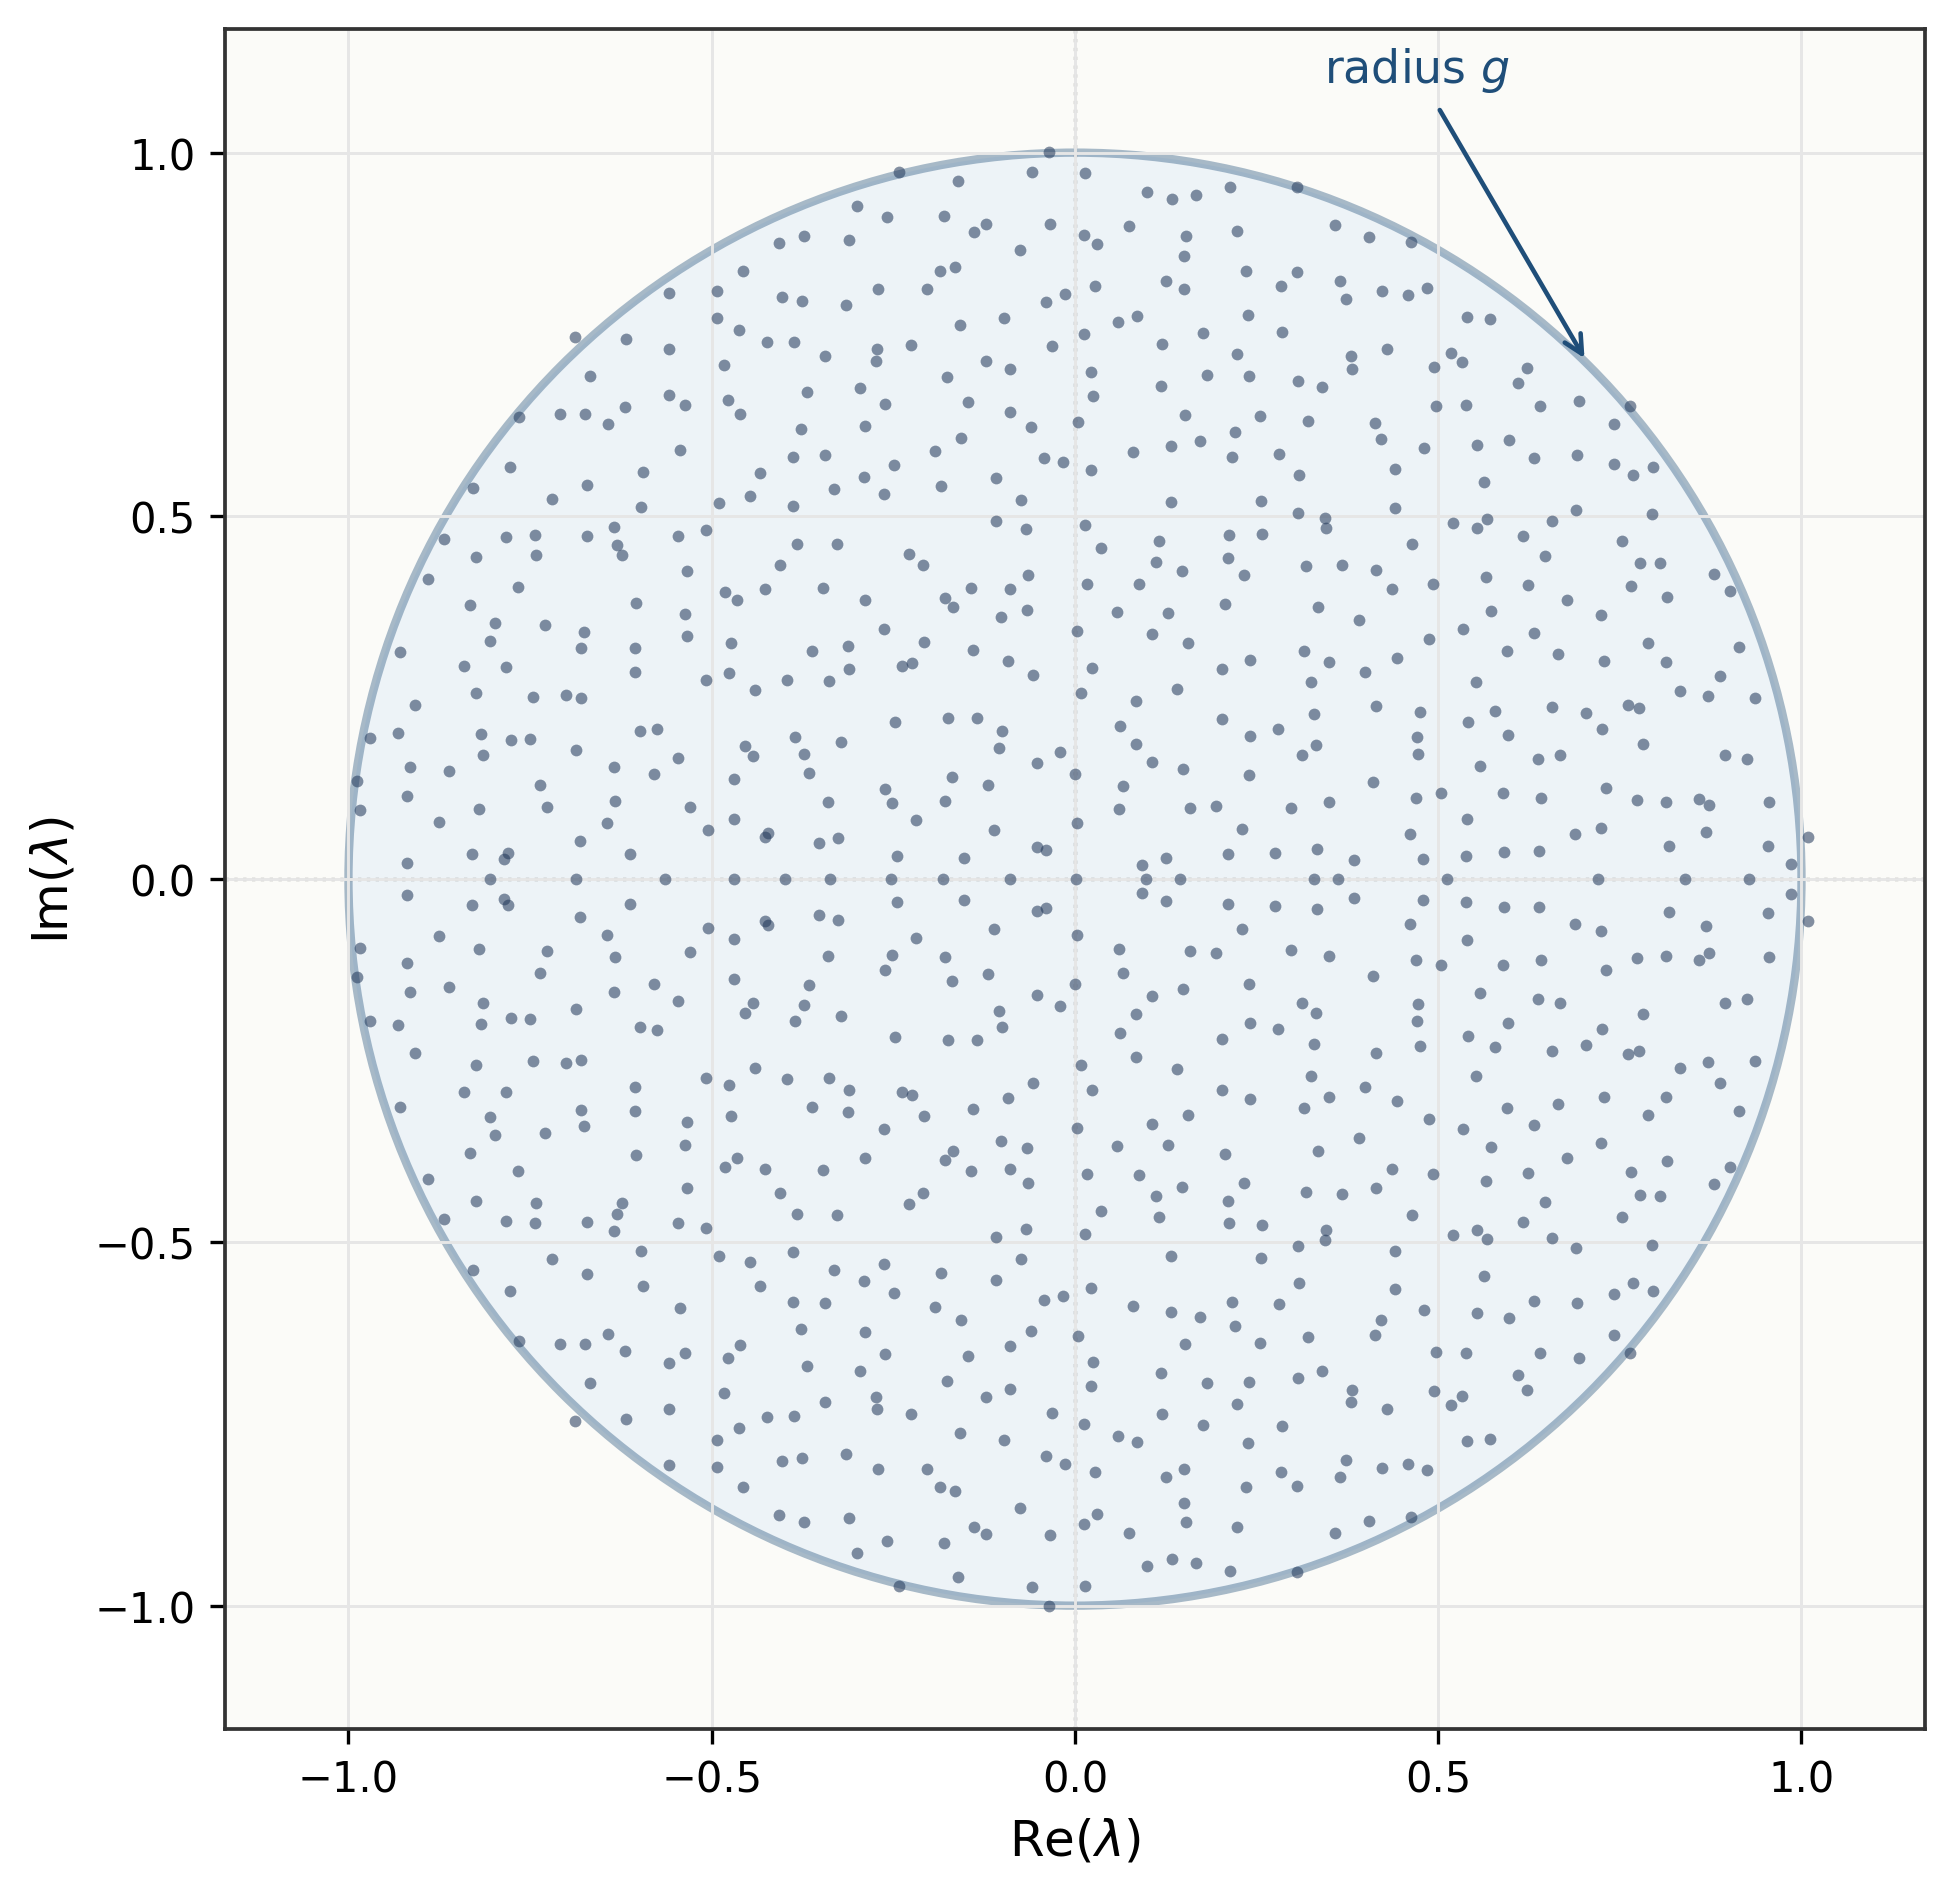
\includegraphics[width=0.5\textwidth]{girko_circular_law.png}
    \caption{Eigenvalues of a random weight matrix $W \in \mathbb{R}^{50\times 50}$
    with $W_{ij}\sim\mathcal{N}(0,g^2/n)$ and $g=1.5$, distributed uniformly on
    the disk $D_g$ in accordance with Girko's circular law.}
    \label{fig:girko}
\end{figure}

The parameter $g$ thus controls the spectral radius $\rho(W) \approx g$ and
determines the effective strength of recurrent feedback, setting the stability
boundary of the network.

%----------------------------------------------------------------------------------------
%	THEORETICAL ANALYSIS
%----------------------------------------------------------------------------------------

\section{Theoretical Analysis}

\subsection{Fixed-Point Analysis of the Undriven Network}

We first analyze the autonomous ($\mathbf{b}=0$, $A=0$) fixed-weight network,

\begin{equation}
    \tau \dot{\mathbf{x}} = -\mathbf{x} + \tanh(W\mathbf{x}).
\end{equation}

Since $\tanh(0)=0$, the origin is always an equilibrium: $\mathbf{x}^* = \mathbf{0}$.
Linearizing at $\mathbf{x} = 0$ using $\tanh'(0) = 1$ gives the Jacobian

\begin{equation}
    J(0) = \frac{1}{\tau}(-I + W).
\end{equation}

Each eigenvalue $\lambda$ of $W$ corresponds to a Jacobian eigenvalue

\begin{equation}
    \mu = \frac{\lambda - 1}{\tau}.
\end{equation}

By Girko's circular law, the eigenvalues of $W$ approximately fill the disk
$|\lambda| \leq g$, so the Jacobian eigenvalues fill the shifted disk
$|\tau\mu + 1| \leq g$.  The rightmost point of this disk lies at

\begin{equation}
    \mathrm{Re}(\mu)_{\max} \approx \frac{g-1}{\tau}.
\end{equation}

Consequently, for $g < 1$ every Jacobian eigenvalue has strictly negative real part
and the origin is a linearly stable equilibrium: small perturbations decay back to
$\mathbf{x}=0$.  For $g > 1$, some Jacobian eigenvalues cross the imaginary axis and
the origin becomes unstable; perturbations can be amplified by recurrent feedback,
giving rise to sustained oscillations or chaotic activity as studied in
\cite{sompolinsky1988chaos}.  The value $g = 1$ is thus a bifurcation point for the
autonomous network.

\subsection{Stability and Existence Under Periodic Drive}

With a periodic external drive $\mathbf{b}(t) = A\sin(\omega t + \boldsymbol{\phi})$,
the autonomous equilibrium is replaced by a driven trajectory $\mathbf{x}^*(t)$.
Perturbations $\delta\mathbf{x}$ around $\mathbf{x}^*(t)$ satisfy the variational
equation

\begin{equation}
    \tau\,\dot{\delta\mathbf{x}} = \bigl[-I + D(t)W\bigr]\delta\mathbf{x},
    \label{eq:variational}
\end{equation}

where

\begin{equation}
    D(t) = \operatorname{diag}\!\bigl(\operatorname{sech}^2(W\mathbf{x}^*(t) + \mathbf{b}(t))\bigr)
\end{equation}

is the diagonal matrix of pointwise activation derivatives evaluated on the driven
trajectory.  The effective recurrent matrix is therefore $D(t)W$, not $W$ itself.

Since $d_i(t) = D_{ii}(t) = \operatorname{sech}^2(h_i(t)) \in (0,1]$ for all $i$ and
$t$, we have the bound $\rho(D(t)W) \leq \|D(t)\|_{\infty}\,\rho(W) \leq \rho(W)$.
For $g < 1$ this gives $\rho(D(t)W) < 1$, which means the Poincar\'{e} map of the
periodically forced $\mathbf{x}$-subsystem is a strict contraction.  By the Banach
fixed-point theorem, there is a unique, globally attracting periodic orbit at frequency
$\omega$, justifying the use of the averaging method in the next section.

\subsection{Oja Plasticity on the Slow Manifold}

The key timescale separation is $\eta\tau = 0.01 \ll 1$: activity relaxes on
timescale $\tau = 1$ while weights evolve on timescale $1/\eta = 100$.  On the fast
(activity) timescale, $W$ is approximately constant, so $\mathbf{x}(t)$ settles to
its unique periodic orbit $\mathbf{x}(t; W)$ determined by the current weight matrix.
Averaging the Oja rule \eqref{eq:oja} over one drive period
$T_{\mathrm{avg}} = 2\pi/\omega$ gives the slow-manifold dynamics

\begin{equation}
    \dot{W}_{ij} \approx \eta\bigl[C_{ij}(W) - C_{ii}(W)\,W_{ij}\bigr] - \lambda W_{ij},
    \label{eq:slow}
\end{equation}

where

\begin{equation}
    C(W) = \frac{1}{T_{\mathrm{avg}}}\int_0^{T_{\mathrm{avg}}}
    \mathbf{x}(t;W)\,\mathbf{x}(t;W)^T\,dt
\end{equation}

is the time-averaged activity correlation matrix.  Setting \eqref{eq:slow} to zero
gives the fixed point condition

\begin{equation}
    W_{ij}^* = \frac{\eta\,C_{ij}(W^*)}{\eta\,C_{ii}(W^*) + \lambda}.
    \label{eq:wstar}
\end{equation}

For fixed (non-adapting) $\mathbf{x}(t) = \mathbf{x}$, equation \eqref{eq:wstar}
reduces exactly to

\begin{equation}
    W_{ij}^* = \frac{\eta\,x_i x_j}{\eta\,x_i^2 + \lambda} = u_i x_j, \qquad
    u_i = \frac{\eta x_i}{\eta x_i^2 + \lambda},
\end{equation}

confirming that the Oja fixed point is rank-one whenever the driving activity is
constant — without any small-parameter approximation.

For sinusoidal drive at frequency $\omega$, every neuron responds at the same
frequency: $x_i(t) \approx r_i\sin(\omega t + \theta_i)$.  The time-averaged
correlation matrix is then

\begin{equation}
    C_{ij}(W) \approx \tfrac{1}{2} r_i r_j \cos(\theta_i - \theta_j),
\end{equation}

which is rank at most one.  Consequently $W^* \approx (\eta/\lambda)\,\mathbf{r}\mathbf{r}^T$
(up to diagonal factors), and the spectral radius satisfies

\begin{equation}
    \rho(W^*) \approx \frac{\eta}{\lambda}\|\mathbf{r}\|^2.
\end{equation}

Since $\|\mathbf{r}\|$ itself grows with $\rho(W)$ — stronger recurrent feedback
entrains the drive more effectively — this is a self-reinforcing feedback loop with
no finite fixed point.  A self-consistent ceiling is reached only when neuron
saturation limits $\|r\|$: in the fully entrained limit $\langle x_i^2\rangle \to 1$
gives

\begin{equation}
    \rho(W^*) \to \frac{n\,\eta}{\eta + \lambda} = \frac{50 \times 0.01}{0.011} \approx 45.5,
\end{equation}

consistent with the observed saturation at $\rho(W^*) \approx 43$--$45$.

\subsection{Effective Random-Matrix Gain Under Drive}

Although the nominal spectral radius $\rho(W)$ characterizes the initial random
matrix, the stability of the \emph{driven} system is governed by $\rho(D(t)W)$, the
spectral radius of the effective recurrent matrix $D(t)W$.  Because the entries of
$D(t)W$ are $d_i(t) W_{ij}$, and $W_{ij}$ has variance $g^2/n$, conditional on
$D(t)$ we have

\begin{equation}
    \mathrm{Var}\bigl((D(t)W)_{ij}\bigr) = \frac{g^2\,d_i(t)^2}{n}.
\end{equation}

Applying Girko's law to the row-inhomogeneous matrix $D(t)W$ motivates the heuristic
effective gain

\begin{equation}
    g_{\mathrm{eff}}(t) \approx \frac{\|W(t)\|_F}{\sqrt{n}}\sqrt{\frac{1}{n}\sum_{i=1}^n d_i(t)^2},
    \label{eq:geff}
\end{equation}

where $\|W\|_F/\sqrt{n}$ replaces $g$ for non-stationary $W(t)$.  When neurons are
unsaturated ($d_i \approx 1$), $g_{\mathrm{eff}} \approx g$.  Under strong periodic
drive, neurons saturate ($|h_i| \to \infty$, $d_i \to 0$), pulling $g_{\mathrm{eff}}$
below $g$ regardless of how large $\rho(W)$ becomes.

%----------------------------------------------------------------------------------------
%	NUMERICAL RESULTS
%----------------------------------------------------------------------------------------

\section{Numerical Results}

All simulations use networks of $n = 50$ neurons with $\tau = 1$, $\eta = 0.01$,
$\lambda = 0.001$, sinusoidal drive amplitude $A = 1$, and frequency $\omega = 1$
unless otherwise specified.  Random phase offsets $\phi_i \sim \mathrm{Uniform}(0,2\pi)$
are drawn independently for each neuron so that the population-averaged input
correlation matrix is not trivially rank-one by construction.  Results are averaged
over 5 random seeds with error bars showing one standard deviation.

\subsection{Oja Learning Does Not Self-Organize to the Edge of Chaos}

A frequently cited motivation for studying local learning rules in recurrent networks
is the conjecture that such rules might spontaneously drive the network toward a
critical operating point near $\rho(W) \approx 1$ (the edge of chaos).  To test
this, we sweep initial spectral radii $g_0 \in \{0.3, 0.5, 0.7, 1.0, 1.5, 2.0, 2.5\}$
and run the full coupled system

\begin{align}
    \tau \dot{x}_i &= -x_i + \tanh\!\Bigl(\textstyle\sum_j W_{ij}x_j + A\sin(\omega t + \phi_i)\Bigr), \nonumber\\
    \dot{W}_{ij} &= \eta\,x_i(x_j - x_i W_{ij}) - \lambda W_{ij},
\end{align}

for $T = 400$ time units under both sinusoidal drive ($A=1$) and autonomous dynamics
($A=0$).

\begin{figure}[H]
    \centering
    
\includegraphics[width=0.75\textwidth]{spectral_radius_trajectories.png}
    \caption{Spectral radius $\rho(W(t))$ over time for all initial conditions $g_0$
    under sinusoidal drive (top) and autonomous dynamics (bottom).  Under drive,
    $\rho(W)\to 45$ regardless of $g_0$.  Without drive, a clean bifurcation at
    $g_0 = 1$ is visible.}
    \label{fig:rho_traj}
\end{figure}

Under sinusoidal drive, $\rho(W) \to 45$ for every initial $g_0$, with all
trajectories converging within $T \approx 150$ time units (Figure~\ref{fig:rho_traj}).
The drive erases all memory of the initial condition.  The autonomous system ($A=0$)
does exhibit a clean bifurcation at $g_0 = 1$, but the addition of periodic input
unfolds this bifurcation, removing the stable branch near $\rho(W) = 1$.  The
mechanism is the self-reinforcing feedback loop derived in Section~4.3: sinusoidal
drive creates a persistent rank-one correlation structure that Oja amplifies until
neuron saturation provides a ceiling.

\subsection{Edge-of-Chaos Optimality for Signal Reconstruction}

Although Oja learning does not maintain the network near the edge of chaos, the
initial spectral radius $g$ still determines the quality of signal reconstruction
during the early learning transient.  For each $g_0$, we run the driven Oja system
for $T = 80$ time units — long enough for activity transients to decay (since $\tau=1$)
but short enough that Oja has not yet fully saturated the network
($\rho(W) \approx 10$--$20$) — and fit a linear readout to reconstruct
$y(t) = \sin(\omega t)$ from the activity history $X \in \mathbb{R}^{T/dt \times n}$:

\begin{equation}
    \mathbf{c}^* = \arg\min_{\mathbf{c}}\,\|X\mathbf{c} - \mathbf{y}\|^2,
    \qquad
    R^2 = 1 - \frac{\|X\mathbf{c}^* - \mathbf{y}\|^2}{\mathrm{Var}(\mathbf{y})}.
\end{equation}

\begin{figure}[H]
    \centering
    
\includegraphics[width=0.7\textwidth]{r2_vs_g.png}
    \caption{Signal reconstruction $R^2$ as a function of initial spectral radius $g_0$.
    The peak near $g_0 \approx 0.9$--$1.0$ reflects the richest transient activity
    at the edge of chaos.  Mean $\pm$ one standard deviation across 5 seeds.}
    \label{fig:r2_vs_g}
\end{figure}

$R^2$ peaks at $g_0 \approx 0.9$--$1.0$, reaching $R^2_{\max} \approx 0.81 \pm 0.06$,
and falls to $R^2 \approx 0.22$ at $g_0 = 3.0$ (Figure~\ref{fig:r2_vs_g}).  Networks
initialized at the edge of chaos produce the richest activity during the learning
transient, enabling more accurate reconstruction before Oja saturation degrades the
signal diversity.  This is consistent with the theoretical picture from reservoir
computing, where proximity to the edge of chaos maximizes the effective dimensionality
of the network's response \cite{sompolinsky1988chaos}.

\subsection{Frozen Random Reservoir Outperforms Oja-Learned Weights}

To assess the value of Oja learning directly, we compare to a frozen random reservoir.
For each $g_0$, we hold the weights fixed ($\eta = 0$) and fit a ridge-regression
readout with regularization $\alpha = 10^{-3}$:

\begin{equation}
    \mathbf{c}^* = (X^TX + \alpha I)^{-1}X^T \mathbf{y}.
\end{equation}

\begin{figure}[H]
    \centering
    
\includegraphics[width=0.7\textwidth]{r2_baseline_vs_oja.png}
    \caption{Comparison of signal reconstruction $R^2$ for Oja-learned weights
    (solid) versus a frozen random reservoir with ridge regression (dashed).  The
    frozen reservoir achieves $R^2 \approx 1.0$ for all $g_0$; Oja learning is
    consistently worse.}
    \label{fig:r2_comparison}
\end{figure}

The frozen reservoir achieves $R^2 \approx 1.0$ for every $g_0$
(Figure~\ref{fig:r2_comparison}).  This is not a trivial result: even a static random
matrix, when driven by $A\sin(\omega t)$, projects the input into a
high-dimensional space from which the target frequency can always be recovered by a
linear readout.  Oja learning is counterproductive: it drives $\rho(W) \to 45$,
saturating the $\tanh$ nonlinearity and destroying the activity diversity that makes
reconstruction easy.  The frozen network retains this diversity for all $g_0$.

\subsection{Input Structure Drives Rank Collapse}

The slow-manifold analysis (Section~4.3) predicts that rank collapse is tied to the
rank of $C(W)$, not to the learning rule itself.  We test this by replacing the
sinusoidal drive with three alternatives:

\begin{itemize}
    \item \emph{Quasi-periodic:} $A/\sqrt{3}\sum_{k=1}^3 \sin(\omega_k t + \phi_i)$,
          with $\omega_1 = 1$, $\omega_2 = \varphi$ (golden ratio), $\omega_3 = \sqrt{2}$
          (mutually incommensurate frequencies).
    \item \emph{White noise:} $\xi_i(t) \sim \mathcal{N}(0, A^2/2)$ drawn independently
          for each neuron at each timestep, matched in RMS power to the sinusoidal drive.
    \item \emph{Zero drive:} $A = 0$ (autonomous network).
\end{itemize}

\begin{figure}[H]
    \centering
    
\includegraphics[width=0.7\textwidth]{correlation_rank_by_drive.png}
    \caption{Rank of the rolling activity correlation matrix $\hat{C}$ over time for
    sinusoidal drive (left) and white noise drive (right), at $g = 1.0$.  Sinusoidal
    drive collapses the rank to 1 within $T \approx 50$; white noise preserves full rank.}
    \label{fig:rank_collapse}
\end{figure}

For $g < 1$ (stable regime), white noise keeps $\mathrm{rank}(\hat{C}) \approx n$ and
prevents rank collapse entirely: $\rho(W) \to 0$ and the participation ratio
$\mathrm{PR}(W) \approx 36$ (Figure~\ref{fig:rank_collapse}).  The isotropic structure
of white noise gives $C \approx \sigma^2 I$, so $W^* \approx (\eta\sigma^2/\lambda) I$
is full-rank with bounded spectral radius.  Sinusoidal drive collapses
$\mathrm{rank}(\hat{C}) \to 1$ within $T \approx 50$ and $\rho(W) \to 43$ regardless
of the initial $g_0$.

For $g > 1.5$ (chaotic regime), even white noise causes collapse, because the dominant
Lyapunov mode of the chaotic network creates its own rank-one correlation structure
that Oja then amplifies.  Thus the precise criterion for rank collapse is: structured
periodic input \emph{in the stable regime}; in the chaotic regime, collapse is
generic.  Quasi-periodic drive with three incommensurate frequencies collapses $\rho(W)$
almost as strongly as a single sinusoid, suggesting that the number of active
spectral modes matters less than whether any periodic structure is present.

\subsection{Effective Gain Is Self-Regulated by Saturation}

We validate the heuristic \eqref{eq:geff} in two complementary experiments.

\textbf{Experiment A (Oja dynamics).}  We track $g_{\mathrm{eff}}(t)$ during Oja
learning alongside $\rho(W(t))$ for sinusoidal and white noise drives.  Under sinusoidal
drive, $\rho(W) \to 43$ but every neuron saturates ($|h_i| \to \infty$), so
$d_i = \operatorname{sech}^2(h_i) \to 0$ and $g_{\mathrm{eff}} \to 0$.  The Oja fixed
point is a \emph{maximally saturated} state: the linearized perturbation dynamics
\eqref{eq:variational} are always stable despite the exploding nominal spectral radius.

\textbf{Experiment C (static scan, frozen weights).}  We hold $\eta = 0$ and scan
$g \in [0.1, 3.0]$ with sinusoidal drive, averaging $g_{\mathrm{eff}}$ and $\rho(D(t)W)$
over the steady-state window $t \in [210, 300]$.

\begin{figure}[H]
    \centering
    
\includegraphics[width=0.7\textwidth]{geff_static_scan.png}
    \caption{Time-averaged effective gain $g_{\mathrm{eff}}$ (blue circles) and direct
    $\rho(D(t)W)$ (orange squares) versus nominal $g$ for frozen weights under sinusoidal
    drive.  The dotted diagonal shows the no-saturation baseline $g_{\mathrm{eff}} = g$.
    The heuristic tracks $\rho(DW)$ within 5\% across all $g$.  The $g_{\mathrm{eff}} = 1$
    stability crossing occurs at $g \approx 1.5$, shifted right of the Girko prediction $g=1$.}
    \label{fig:geff_scan}
\end{figure}

The heuristic tracks $\rho(D(t)W(t))$ within 5\% across all tested $g$
(Figure~\ref{fig:geff_scan}).  The $g_{\mathrm{eff}} = 1$ crossing occurs at
$g \approx 1.5$: sinusoidal drive saturates neurons enough to reduce the effective
gain by approximately 33\%, shifting the effective stability boundary substantially
above the Girko prediction $g = 1$.

\subsection{Critical Slowing Down at the Phase Transition}

Independent evidence for the $g = 1$ phase transition comes from the autonomous
discrete map $h_{t+1} = Wf(h_t)$.  A small perturbation $\delta h(0)$ evolves as
$\|\delta h(t)\| \sim \|\delta h(0)\| e^{\lambda_1 t}$ in the linear regime, where
$\lambda_1$ is the largest Lyapunov exponent (LLE), estimated by a 300-step warmup
followed by 800-step single-vector power iteration.  For $\lambda_1 < 0$ the
relaxation time is $\tau_{\mathrm{relax}} = -1/\lambda_1$; for $\lambda_1 > 0$ no
relaxation time is defined.

\begin{figure}[H]
    \centering
    
\includegraphics[width=0.85\textwidth]{critical_slowing_down.png}
    \caption{Left: relaxation time $\tau_{\mathrm{relax}} = -1/\lambda_1$ versus
    $g$ for the autonomous discrete map.  Right: perturbation divergence curves for
    representative $g$ values after warmup to the attractor.  $\tau_{\mathrm{relax}}$
    diverges as $g \to 1^-$.}
    \label{fig:csd}
\end{figure}

\begin{table}[H]
    \centering
    \caption{Largest Lyapunov exponent and relaxation time for selected $g$ values.}
    \label{tab:lle}
    \begin{tabular}{lrr}
    \toprule
    $g$ & $\lambda_1$ (nats/step) & $\tau_{\mathrm{relax}}$ (steps) \\
    \midrule
    $0.30$ & $-1.20$ & $0.8$ \\
    $0.70$ & $-0.35$ & $2.9$ \\
    $0.90$ & $-0.10$ & $10.8$ \\
    $1.00$ & $-0.005$ & $\approx 350$ \\
    $2.00$ & $+0.10$  & (chaotic) \\
    \bottomrule
    \end{tabular}
\end{table}

Table~\ref{tab:lle} and Figure~\ref{fig:csd} show that $\tau_{\mathrm{relax}}$
diverges as $g \to 1^-$, which is the defining signature of a continuous (second-order)
phase transition \cite{guckenheimer1983nonlinear}.  At $g = 1$ the network has no
preferred timescale for returning to equilibrium: small disturbances persist
arbitrarily long.  This critical slowing down is observable independently of the sign
of the LLE and provides a physically clean signature of the edge-of-chaos transition.

%----------------------------------------------------------------------------------------
%	DISCUSSION AND CONCLUSION
%----------------------------------------------------------------------------------------

\section{Discussion and Conclusion}

We have studied a recurrent network in which both activity and weights evolve
simultaneously under Oja-type plasticity with sinusoidal drive.  The main findings are
as follows.

\textbf{Oja learning drives collapse, not criticality.}  Contrary to the
self-organization-to-criticality conjecture, Oja learning under sinusoidal drive drives
$\rho(W) \to 45$ regardless of the initial spectral radius $g_0$.  The mechanism is
a self-reinforcing feedback loop: periodic drive entrains all neurons at the same
frequency, making the activity correlation matrix rank-one, which Oja then amplifies
until neuron saturation provides a ceiling.  The ceiling is determined by the
self-consistent equation $\rho(W^*) \approx n\eta/(\eta + \lambda)$, independent of $g_0$.

\textbf{Initial $g$ still matters for readout quality.}  Even though Oja learning
erases the memory of $g_0$ in the weights, $g_0$ determines the quality of signal
reconstruction during the early learning transient.  $R^2$ peaks near $g_0 \approx 1$
and falls monotonically for $g_0 > 1.5$, confirming that proximity to the edge of
chaos maximizes the activity diversity exploited by the linear readout.

\textbf{Frozen reservoirs outperform learned weights.}  A static random reservoir with
ridge regression achieves $R^2 \approx 1.0$ for all $g_0$, while Oja-learned weights
degrade reconstruction by destroying activity diversity.  This suggests that for the
specific task of periodic signal reconstruction, Oja plasticity is harmful rather than
helpful.

\textbf{Rank collapse requires structured periodic input in the stable regime.}
White noise drive (matched in RMS power to the sinusoidal drive) keeps the correlation
matrix full-rank and prevents both rank collapse and spectral radius growth for $g < 1$.
This isolates the cause of collapse as the temporal structure of the input — its
periodicity — rather than its amplitude.  In the chaotic regime ($g > 1.5$), collapse
occurs regardless of input structure, driven by the dominant Lyapunov mode.

\textbf{The effective gain provides a better stability predictor than $g$.}
The heuristic $g_{\mathrm{eff}}$ tracks $\rho(D(t)W)$ within 5\% and reveals that
sinusoidal drive shifts the effective stability boundary from $g = 1$ to $g \approx 1.5$
due to neuron saturation.  During Oja learning, $g_{\mathrm{eff}} \to 0$ as the
network saturates, confirming that the Oja fixed point is dynamically stable despite
the large nominal spectral radius.

\textbf{Seizure connection and open questions.}  The key experimental prediction is:
rhythmic periodic input is necessary for Oja-driven rank collapse in stable networks,
while random input is not sufficient.  This suggests that pathological periodicity —
rather than high firing rates alone — may be the mechanistically important feature of
seizure-like activity that drives network-level dimensionality collapse via Hebbian
plasticity.

Several questions remain open.  A full stability analysis of the self-consistent fixed
point $W^* = \eta C(W^*)/(\eta C(W^*) + \lambda I)$ would clarify whether the
$\rho(W) \to \infty$ trajectory is the unique attractor under sinusoidal drive, or
whether bounded fixed points exist at large $n$.  A precise criterion
characterizing exactly which input power spectra lead to rank collapse would sharpen
the connection to the seizure hypothesis and potentially suggest intervention strategies.

\bibliographystyle{plain}
\bibliography{references}

\end{document}
